\FloatBarrier
\begin{figure}[!h]
\centering
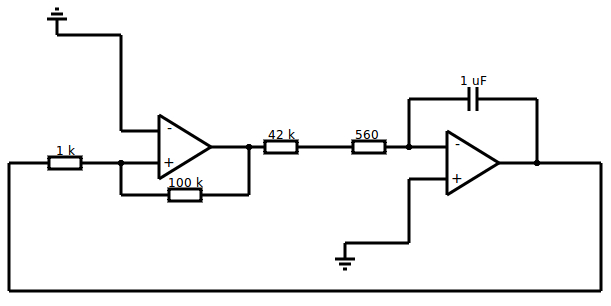
\includegraphics[scale=0.6]{../Grafiken/Funktionsgenerator_real.jpg}
\caption{Die verwendete Schaltung eines 
Funktionsgenerators. Es wurden zwei  zusätzliche Widerstände in Reihe 
(dargestellt ist nur die Summe beider Widerstände) geschaltet, um 
die Eingangspannung des zweiten Operationsverstärkers zu verringern.
\label{fig:funktionsgenerator_real}}
\end{figure}
\FloatBarrier